\begin{frame}{Global Picture}
\centering
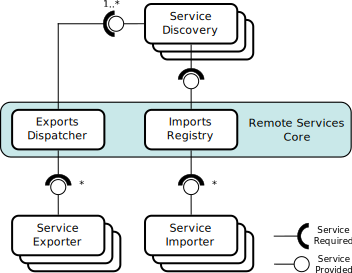
\includegraphics{../imgs/rs_arch}
\end{frame}

\begin{frame}{Remote Services Services}
\begin{exampleblock}{Note}
All services names are declared in \texttt{pelix.remote}
\end{exampleblock}

\begin{block}{Core Services}
\begin{small}
\begin{tabular}{rp{.55\textwidth}}
\texttt{\scriptsize SERVICE\_DISPATCHER} & Read-only access to the list of export endpoints \\
\texttt{\scriptsize SERVICE\_DISPATCHER\_SERVLET} & Utility methods for HTTP-based discovery \\
\texttt{\scriptsize SERVICE\_REGISTRY} & Write-only access to the list of import endpoints \\
\end{tabular}
\end{small}
\end{block}

\begin{block}{Import/Export Services}
\begin{small}
\begin{tabular}{rp{.45\textwidth}}
\texttt{\scriptsize SERVICE\_EXPORT\_PROVIDER} & Notified by the dispatcher to create export endpoints \\
\texttt{\scriptsize SERVICE\_EXPORT\_ENDPOINT\_LISTENER} & Notified of new export endpoints \\
\texttt{\scriptsize SERVICE\_IMPORT\_ENDPOINT\_LISTENER} & Notified of new import endpoints \\
\end{tabular}
\end{small}
\end{block}
\end{frame}

\begin{frame}{API: \texttt{SERVICE\_DISPATCHER}}
\begin{block}{Description}
\begin{small}
Service implemented by \texttt{Dispatcher} in the \texttt{dispatcher} module.
It notifies the exporters for each \texttt{ServiceReference} associated to export properties.
It then keeps track of the \texttt{ExportEndpoint} created by the exporters.
\end{small}
\end{block}

\begin{block}{Public methods}
\begin{small}
\begin{tabular}{p{13em} p{.5\textwidth}}
\texttt{get\_endpoint(uid)} & Returns the \texttt{ExportEndpoint} associated to the given UID \\
\hline
\texttt{get\_endpoints( kind=None, name=None)} & Retrieves all \texttt{ExportEndpoint} matching the given kind and/or name \\
\end{tabular}
\end{small}
\end{block}
\end{frame}

\begin{frame}{API: \texttt{SERVICE\_DISPATCHER\_SERVLET}}
\begin{block}{Description}
\begin{small}
Service implemented by \texttt{RegistryServlet} in the \texttt{dispatcher} module.
It allows to grab the description of exported endpoints in JSON format \textit{via} a GET request.
It also supports the update of an imported endpoint \textit{via} a POST request.
The service can be used internally to send those requests.
\end{small}
\end{block}

\begin{block}{Public methods}
\begin{small}
\begin{tabular}{p{.3\textwidth} p{.6\textwidth}}
\texttt{get\_access()} & Returns the HTTP port and path to access the servlet \\
\hline
\texttt{grab\_endpoint( host, port, path, uid)} & Get the description of an exported endpoint from a framework\\
\hline
\texttt{send\_discoverted( host, port, path)} & Sends a \textit{discovered} POST request to a framework \\
\end{tabular}
\end{small}
\end{block}
\end{frame}

\begin{frame}{API: \texttt{SERVICE\_REGISTRY}}
\begin{block}{Description}
\begin{small}
Service implemented by \texttt{ImportsRegistry} in the \texttt{registry} module.
Keeps track of all discovered exported endpoints as \texttt{ImportedEndpoint}s, after having been notified by discovery services.
Notify importers of known endpoints and let them decide whether to import the service or not.
\end{small}
\end{block}

\begin{block}{Public methods}
\begin{small}
\begin{tabular}{lp{.55\textwidth}}
\texttt{add(endpoint)} & Registers a new \texttt{ImportEndpoint} \\
\hline
\texttt{update(uid, new\_props)} & Updates the properties of a known \texttt{ImportEndpoint}\\
\hline
\texttt{remove(uid)} & Unregisters a known \texttt{ImportEndpoint}\\
\hline
\texttt{lost\_framework(uid)} & Unregisters all \texttt{ImportEndpoint} associated to a framework\\
\end{tabular}
\end{small}
\end{block}
\end{frame}
